\subsection{Práctica N° 5: Realimentación}

\subsubsection{Amplificador realimentado negativamente}

\begin{table}[h!]
\centering
\begin{tabular}{|c|c|c|c|c|c|}
\hline
\textbf{\(Vg[V]\)} & \textbf{\(\varDelta Vg[V]\)} & \textbf{\(Vi[V]\)} & \textbf{\(\varDelta Vi[V]\)} & \textbf{\(Rp[\Omega]\)} & \textbf{\(\varDelta Rp[\Omega]\)} \\ \hline
0.2 & 0.02 & 0.06 & 0.01 & 100000 & 5000 \\ \hline
\end{tabular}
\caption{Mediciones para calcular la impedancia de entrada del amplificador con realimentación negativa}
\label{tab:med-impedancia-entrada-amplificador-realimentacion-negativa}
\end{table}


\begin{table}[h!]
\centering
\begin{tabular}{|c|c|c|c|c|c|}
\hline
\textbf{\(Vo_{sc}[V]\)} & \textbf{\(\varDelta Vo_{sc}[V]\)} & \textbf{\(Vo_{cc}[V]\)} & \textbf{\(\varDelta Vo_{cc}[V]\)} & \textbf{\(Rp[\Omega]\)} & \textbf{\(\varDelta Rp[\Omega]\)} \\ \hline
1 & 0.1 & 1 & 0.1 & 1 & 0.05 \\ \hline
\end{tabular}
\caption{Mediciones para calcular la impedancia de salida del amplificador con realimentación negativa}
\label{tab:med-impedancia-salida-amplificador-realimentacion-negativa}
\end{table}

\begin{table}[h!]
\centering
\begin{tabular}{|c|c|c|c|}
\hline
\textbf{\(Vi[V]\)} & \textbf{\(\varDelta Vi[V]\)} & \textbf{\(Vo[V]\)} & \textbf{\(\varDelta Vo[V]\)} \\ \hline
0.16 & 0.01 & 0.72 & 0.02 \\ \hline
\end{tabular}
\caption{Mediciones para calcular la ganancia del amplificador con realimentación negativa}
\label{tab:med-ganancia-amplificador-realimentacion-negativa}
\end{table}

\begin{table}[h!]
\centering
\begin{tabular}{|c|c|c|c|c|c|}
\hline
\textbf{Parámetro} & \textbf{Valor Real} & \textbf{Medición} & \textbf{Incertidumbre} & \textbf{Error Absoluto} & \textbf{Error Relativo} \\ \hline
$Z_i$ & 100000 & 42857.14286 & 12091.29853 & 57142.85714286 & 57.14\% \\ \hline
$z_o$ & 0.17 & 0 & 0.141421356 & 0.17000000 & 100.00\% \\ \hline
$A_b$ & -3.33 & -4.5 & 0.307776806 & 1.17000000 & 35.14\% \\ \hline
$F_L$ & 1.37 & 1 & 0.04 & 0.37000000 & 27.01\% \\ \hline
$F_H$ & 555940 & 588235.2941 & 34602.07612 & 32295.29411765 & 5.81\% \\ \hline
\end{tabular}
\caption{Modelo dinámico y frecuencias de corte del amplificador realimentado negativamente}
\label{tab:med-modelo-dinamico-frecuencias-corte-amplificador-realimentado-negativamente}
\end{table}

\begin{ilustracion}[ht]
    \centering
    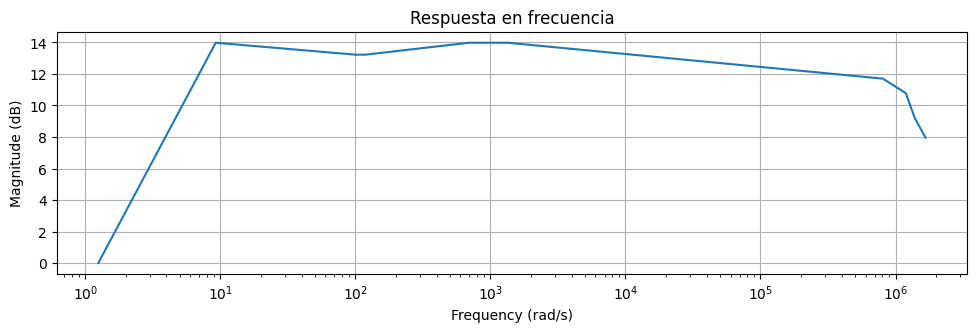
\includegraphics[width=0.8\textwidth]{src/images/resultados/p5/respuesta en frecuencia realimentacion negativa.png}
    \caption{Respuesta en frecuencia Amplificador realimentado negativamente}
    \label{ilus:amplificador-realimentado-negativamente}
\end{ilustracion}

\begin{ilustracion}
    \centering
    \includegraphics[width=0.8\textwidth]{src/images/resultados/p5/superposición respuesta en frecuencia con simulacion.png}
    \caption{Superposición de ganancia en frecuencia Amplificador realimentado negativamente}
    \label{ilus:amplificador-realimentado-negativamente-superposicion}
\end{ilustracion}